\chapter{Ανεπάρκεια Προστασίας των Δεδομένων}

Οι εργασίες για την προστασία των προσωπικών δεδομένων έχουν ξεκινήσει εδώ και αρκετές δεκαετίες. Δυστυχώς, παρά τον σχετικά ορθό σχεδιασμό τους και το μεγάλο μέγεθος των συνόλων δεδομένων που αυτές εφαρμόζονται, η αποκάλυψη και η ταυτοποίηση εγγραφών είναι όπως θα δούμε αναπόφευκτη. 

Στο κεφάλαιο αυτό αναφέρουμε αρχικά περιπτώσεις διαρροής πληροφοριών κατά την επεξεργασία συνόλων δεδομένων. Στη συνέχεια, περιγράφουμε τη λειτουργία βασικών τεχνικών προστασίας και τονίζουμε τα σημεία στα οποία αυτές αποτυγχάνουν.



\section{Παραδείγματα αποκάλυψης πληροφορίας}

Κατά καιρούς έχουν προταθεί αρκετοί, διαφορετικοί μεταξύ τους, ορισμοί για την έννοια της διαρροής και αποκάλυψης πληροφοριών κατά την επεξερασία δεδομένων. 
Η αποκάλυψη σχετίζεται με την απόδοση σημαντικών πληροφοριών σε έναν ερωτώμενο, είτε πρόκειται για ένα άτομο είτε για έναν οργανισμό. Διακρίνουμε τρία είδη αποκάλυψης: όταν το άτομο μπορεί να ταυτοποιηθεί από το σύνολο δεδομένων (αποκαλυψη ταυτότητας), όταν διαρρεύσουν ευαίσθητες πληροφορίες για κάποιο άτομο (αποκάλυψη γνωρίσματος), και όταν τα δημοσιευμένα δεδομένα καθιστούν δυνατό τον ακριβέστερο προσδιορισμό της τιμής κάποιου γνωρίσματος μιας εγγραφής από ό, τι θα ήταν εφικτό (επαγωγική αποκάλυψη).


Παρακάτω κάνουμε μια συλλογή παραδειγμάτων αποκάλυψης και επιθέσεων στα οποία βλέπουμε πως από ένα σύνολο δεδομένων απο το οποίο απουσιάζουν ή αποκρύπτονται προσωπικά στοιχεία, ο επιτιθέμενος καταφέρνει να εξάγει την απαραίτητη πληροφορία ώστε να μπορεί να ταυτοποιηθεί τουλάχιστον ένα άτομο, ή η τιμή ενός ευαίσθητου γνωρίματος μιας εγγραφής, εντός του συνόλου. Τις περισσότερες φορές αυτό γίνεται με τη χρήση βοηθητικών πληροφοριών. Αυτό μπορεί να είναι οποιαδήποτε πρόσθετη πληροφορία που έχει πρόσβαση ο επιτιθέμενος, συμπεριλαμβανομένων παλαιότερων εκδόσεων της αρχικής βάσης δεδομένων. 


\begin{itemize}
   
\item \textbf{Η διαρροή δεδομένων αναζήτησης της $AOL$}\\
Τον Αύγουστο του 2006, η \textlatin{AOL Research} δημοσιεύει σε μια από τις ιστοσελίδες της έναν συμπιεσμένο φάκελο ο οποίος περιείχε 20 εκατομμύρια επερωτήσεις από 650.000 χρήστες. Σε μια προσπάθεια διατήρησης της ιδιωτικότητας, αντικατέστησαν τα ονόματα χρηστών με έναν αριθμό που δημιουργήθηκε τυχαία, ενώ επίσης επεξεργάστηκαν προσεκτικά αποκαλυπτικές επερωτήσεις (παράδειγμα, όταν τα άτομα αναζητούν το δικό τους όνομα ή αριθμό ασφαλείας). Ωστόσο, μπορούσε να εξαχθεί το πλήρες ιστορικό αναζήτησης ενός ατόμου. Αυτό με τη σειρά του, επέτρεπε σε οποιονδήποτε να εντοπίζει τα άτομα με βάση το ιστορικό αναζήτησης και, συνεπώς, να παραβιάσει την ιδιωτικότητά τους. 
Συγκεκριμένα, ερευνητές της \textlatin{New York Times} κατάφεραν να εντοπίσουν ένα άτομο από τα δημοσιευμένα και ανώνυμα αρχεία αναζήτησης, διασταυρώνοντάς τα με λίστες τηλεφωνικών καταλόγων.
Η \textlatin{AOL} αναγνώρισε το λάθος της και αφαίρεσε τα δεδομένα την αμέσως επόμενη ημέρα. Ωστόσο, η ζημιά είχε ήδη γίνει. Τα δεδομένα αναδιανεμήθηκαν από άλλους και μπορούν ακόμη και σήμερα να μεταφορτωθούν από \textlatin{mirror sites}.
\begin{figure} [h!]
\begin{center}
  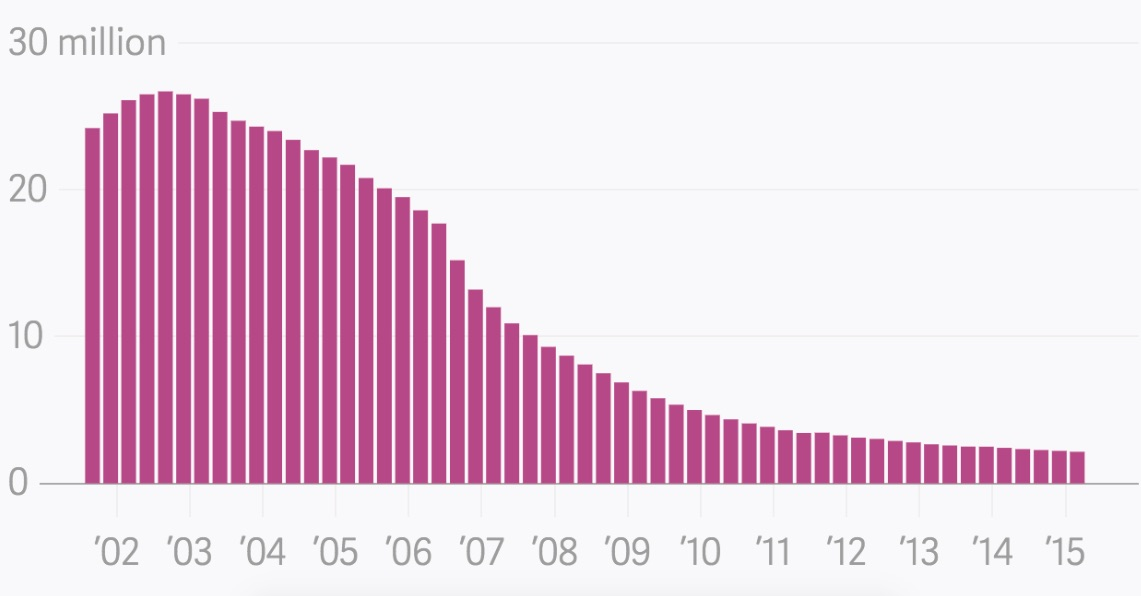
\includegraphics[scale=0.3]{images/AOL.jpg}
  \caption{Χρήστες $AOL$ από το 2002}
  %\label{fig:boat1}
  \end{center}
\end{figure}


Εντούτοις, δεν είναι σωστό να θεωρούμε ότι η προστασία της ιδιωτικότητας ενός συνόλου δεδομένων είναι δύσκολο έργο, επηρεασμένοι από το παραπάνω γεγονός. Αυτό συνέβει επειδή δεν δόθηκε ουσιαστική προσοχή στην ανωνυμοποίηση των αποτελεσμάτων αναζήτησης, πράγμα που συμπεραίνουμε από την άμεση απομάκρυνση από την εταιρία του υπευθύνου της κοινοποίησης των δεδομένων. Επιπλέον, ο προϊστάμενος της \textlatin{AOL Research} απολύεται ενώ ο \textlatin{CTO} παραιτήθηκε. Τελικά το γεγονός οδήγησε στην άμεση απομάκρυνση πολλών χρηστών, με αποτέλεσμα την επιτάχυνση της ήδη φθίνουσας πορείας της εταιρίας. 


\item \textbf{Διασταύρωση ιατρικών δεδομένων }

Μιά από τις δημοφιλέστερες αναδείξεις παραβίασης είναι η ταυτοποίηση του κυβερνήτη της Μασαχουσέτης σε λίστα ιατρικών δεδομένων. 

Είναι αποδεδειγμένο ότι το 63\% του πληθισμού των Ηνωμένων Πολιτειών μπορεί να ταυτοποιηθεί αν είναι γνωστά μόνο: ο ταχυδρομικός κώδικας, το φύλο και η ημερομηνία γέννησης ενός ατόμου. Σύμφωνα με ένα άρθρο \textlatin{\cite{Sweeney:2001:CDC:935675} }, αν ασκηθεί επίθεση συνδεσιμότητας σε δύο βάσεις δεδομένων που μοιράζονται αυτή την τριάδα γνωρισμάτων, τότε μπορεί να ταυτοποιηθεί μια τουλάχιστον εγγραφή. Συγκεκριμένα, στο πείραμα χρησιμοποιήθηκε ως πρώτη βάση ο κατάλογος ψηφοφόρων του \textlatin{Cambridge} και ως δεύτερη η βάση δεδομένων υγείας του \textlatin{ Massachusetts Group Insurance Commission (GIC)}. Τόσο ο κατάλογος ψηφοφόρων όσο και η βάση δεδομένων υγείας κάνουν χρήση των γνωρισμάτων \{ T.K, φύλο, ημερομηνία γέννησης \}, και αφού συνδυάστηκαν δυο εγγραφές, μια σε κάθε βάση, ταυτοποιήθηκαν τα στοιχεία του πρώην κυβερνήτη \textlatin{William Weld}. 

\begin{figure} [h!]
\begin{center}
  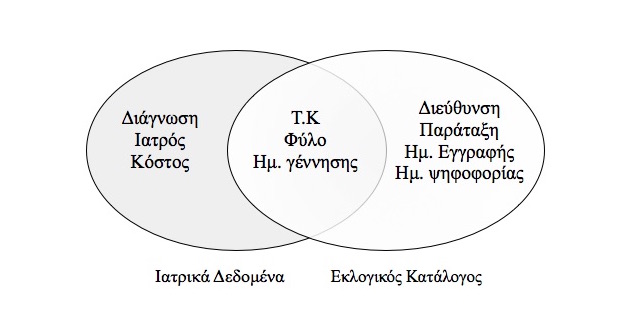
\includegraphics[scale=0.55]{images/TK.jpg}
  \caption{Συνδιασμός κοινών γνωρισμάτων}
  %\label{fig:boat1}
  \end{center}
\end{figure}

Αυτό που προκάλεσε ανησυχία δεν είναι το ότι κάτάφερε να ταυτοποιηθεί ένα διάσημο πρόσωπο συνδυάζοντας τα στοιχεία δυο βάσεων, αλλά ότι τέτοιου τύπου βάσεις, κυρίως με ιατρικά δεδομένα, είχαν ήδη διαμοιραστεί σε εταιρίες και ερευνητές πιστεύοντας λανθασμένα ότι τα δεδομένα είναι ανωνυμοποιημένα. 
Παρόλο που τα σύνολα δεδομένων δεν περιείχαν προσωπικά αναγνωριστικά, όπως το όνομα ή τον αριθμό κοινωνικής ασφάλισης ενός ασθενούς, τα άτομα μπορούσαν ακόμα να αναγνωριστούν συνδυάζοντας δύο βάσεις δεδομένων. 
\clearpage




\item \textbf{Το βραβείο του 1 εκατομμυρίου της  \textlatin{Netflix}}

Η \textlatin{Netflix} είναι μια εταιρία που παρέχει συνδρομιτικές υπηρεσίες τηλεόρασης σε μορφή \textlatin{on demand}. Για να βελτιώσει τον αλγόριθμο εμφάνισης προτεινόμενων ταινιών, η εταιρία δημοσίευσε αρχικά ένα σύνολο δεδομένων που περιείχε περισσότερες από 100 εκατομμύρια βαθμολογίες ταινιών από 480 χιλιάδες χρήστες σε σχεδόν 18 χιλιάδες τίτλους, και στη συνέχεια προσέφεραν ένα βραβείο αξίας 1 εκατομμυρίου δολαρίων σε εκείνους που θα μπορούσαν να βελτιώσουν το τρέχων σύστημα κατά τουλάχιστον 10\%.
Σε μια προσπάθεια διασφάλισης της ιδιωτικότητας των χρηστών τους, αφαιρούν δεδομένα προσωπικού χαρακτήρα.
Το μόνο που απομένουν είναι οι βαθμολογίες (βαθμολογία μεταξύ 1 και 5), η ημερομηνία που δόθηκε η βαθμολογία, το ανώνυμο αναγνωριστικό του χρήστη που έδωσε την αξιολόγηση και τέλος ο τίτλος της ταινίας που αξιολογήθηκε.
Η \textlatin{Netflix} δήλωσε επίσης ότι το σύνολο που δημοσιεύθκε αποτελούσε λιγότερο από το ένα δέκατο του πλήρους συνόλου δεδομένων και ότι τα δεδομένα είναι διαταραγμένα. 
Επίσης δήλωσε, ότι αυτό το ποσοστό επιλέχτηκε τυχαία.
Στην πραγματικότητα, αν παρατηρήσουμε το πλήθος βαθμολογιών για κάθε χρήστη βλέπουμε ότι ελάχιστοι έχουν βαθμολογήσει κάτω από 20 ταινίες \textlatin{\cite{Narayanan:2008:RDL:1397759.1398064}}. 

\begin{figure} [h!]
\begin{center}
  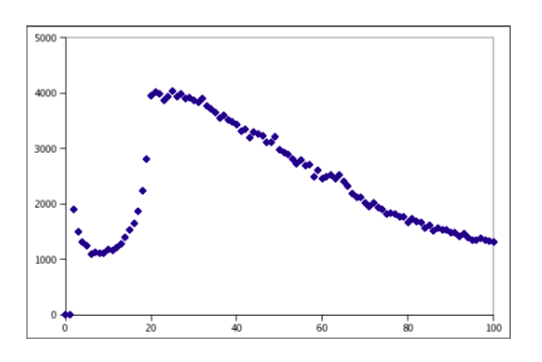
\includegraphics[scale=0.6]{images/Netflix.jpg}
  \caption{Πληθος χρηστών \textlatin{Netflix}, προς πλήθος βαθμολογιών}
  %\label{fig:boat1}
  \end{center}
\end{figure}

Επιπλέον, τέθηκε υπό αμφισβίτηση η υποτιθέμενη διάταραξη των δεδομένων, όταν ταυτοποιήθηκαν δυο συνδρομητές εντός των δεδομένων. O ένας από αυτούς είχε τροποποιημένες 1 από τις 306 αξιολογήσεις ενώ ο άλλος είχε 5 από 229, άρα το ποσοστό θορύβου ήταν ελάχιστο. 
Εδώ βέβαια, είναι σημαντικό να ληφθεί υπόψη ότι το σύνολο δεδομένων δημοσιέυτηκε με σκοπό την ανάπτυξη βελτιωμένων αλγορίθμων. Επομένως αν υπήρχε υπερβολική διαταραχή, θα είχε μειωθεί σημαντικά η χρησιμότητα του συνόλου. 

Το άρθρο του \textlatin{Narayanan} αποδεικνύει ότι απαιτείται ελάχιστη συνδεσιμότητα με εξωτερικά στοιχεία ώστε να ταυτοποιηθεί ένας συνδρομητής. Η σύνδεση στην προκειμένη περίπτωση γίνεται με εγγραφές από την βάση δεδομένων του \textlatin{IMDb}. Μέσα από μόνο 50 εγγραφές, ταυτοποιήθηκαν δυο χρήστες. 

Είναι εύλογο να αναρωτηθεί κάποιος για το αν αξίζει να ανησυχούμε για την ιδιωτικότητα δεδομένων τέτοιου τύπου. Αν όμως αναλογιστούμε το πόσο αποκαλυπτικό για τις πολιτικές πεποιθήσεις ενός ατόμου μπορεί να είναι η προτίμηση ταινιών όπως \textlatin{Fahrenheit 9/11} και \textlatin{Death by China}, συμπεραίνουμε ότι η παροχή προστασίας της ιδιωτικότητας είναι αναγκαία. 

\end{itemize}






\section{Ανεπαρκείς προσεγγίσεις προστασίας}

Ως κριτήρια της αποτελεσματικής ανωνυμοποίησης θωρούνται τα παρακάτω:
\begin{itemize}\label{kri}
\item Μη δυνατότητα εντοπισμού φυσικού προσώπου

\item Μη συνδεσιμότητα μεταξύ καταχωρήσεων που αντιστοιχούν σε ένα πρόσωπο

\item Μη δυνατότητα εξαγωγής συμπερασμάτων σχετικά με ένα φυσικό πρόσωπο.
\end{itemize}



Έχουν παρουσιαστεί κατα καιρούς αρκετές προτάσεις για τη διαφύλαξη της ιδιωτικότητας κατά την ανάλυση δεδομένων. Ωστόσο, οι περισσότερες από αυτές δεν ικανοποιούν τις παραπάνω εγγυήσεις απορρήτου. Αξίζει όμως να αναφερθούν αυτές οι προσπάθειες, διότι οφείλουμε να τονίσουμε ότι η διατήρηση της ιδιωτικότητας μπορεί να είναι ένα δύσκολο έργο με απροσδόκητα προβλήματα.

\begin{itemize}
   
\item \textbf{Επερωτήσεις μεγάλων συνόλων}\\
Μια κοινή ιδέα είναι να απαγορευτεί η εκτέλεση επερωτήσεων σχετικά με ένα συγκεκριμένο άτομο ή ένα μικρό σύνολο ατόμων. Είναι εύκολο να καταλάβουμε ότι αυτή η στρατηγική είναι ανεπαρκής όταν γνωρίζουμε ότι ένα συγκεκριμένο άτομο $X$ είναι στη βάση δεδομένων. Αυτό που μπορούμε να κάνουμε είναι να εφαρμόσουμε δυο «μεγάλες» επερωτήσεις. Η πρώτη, για παράδειγμα, μπορεί να είναι «Πόσα άτομα στη βάση δεδομένων έχουν διαβήτη?» και η δεύτερη «Πόσα άτομα στη βάση δεδομένων, που δεν ονομάζονται $X$, έχουν διαβήτη?». Από τα αποτελέσματα των δυο επερωτήσεων μπορούμε να συμπεράνουμε την κατάσταση του ατόμου $X$. Παρόλο που και οι δυο επερωτήσεις θεωρούνται μεγάλες, παραβιάστηκε η ιδιωτικότητα μιας εγγραφής.

\item \textbf{Έλεγχος Επερωτήσεων}\\
Μια άλλη στρατηγική είναι η αξιολόγηση κάθε επερώτησης στη βάση δεδομένων στο πλαίσιο του ιστορικού των επερωτήσεων, ώστε να προσδιοριστεί εάν μια απάντηση θα ήταν αποκαλυπτική. Εάν η επερώτηση θεωρηθεί ότι παραβιάζει την ιδιωτικότητα, απορρίπτεται και δεν επιστρέφεται απάντηση. Αυτή η μέθοδος μπορεί να χρησιμοποιηθεί για την ανίχνευση της επερώτησης στο προγούμενο παράδειγμα με το αν ένα άτομο Χ έχει ή όχι διαβήτη. Παρόλο που η τεχνική αυτή μπορεί να φαίνεται πολλά υποσχόμενη, η παρακολούθηση όλων των επερωτήσεων είναι υπολογιστικά ανέφικτη \textlatin{\cite{kleinberg1998segmentation}}. Επιπλέον, η ίδια η άρνηση απάντησης σε μιά επερώτηση μπορεί να είναι αποκαλυπτική. Για αυτούς τους λόγους, η παραπάνω προσέγγιση είναι πρακτικά μη εφαρμόσιμη.

\item \textbf{Δειγματοληψία}\\
Η δειγματοληψία μερικές φορές θεωρείται ως πιθανή λύση στο πρόβλημα. Εδώ ένας τυχαίος αριθμός εγγραφών στη βάση δεδομένων θα επιλεγεί τυχαία και οι πληροφορίες τους θα επιστραφούν προς ανάλυση. Ιδιότητες και στατιστικά στοιχεία μπορούν στη συνέχεια να υπολογιστούν στο νέο. Αν γίνει επιλογή ενός αρκετά μεγάλου υποδείγματος τα αποτελέσματα είναι αντιπροσωπευτικά της βάσης ως σύνολο.

Λαμβάνοντας υπόψη ότι το υποσύνολο είναι συνήθως μικρό σε σύγκριση με το μέγεθος της βάσης δεδομένων, είναι απίθανο να επιλεγεί μια συγκεκριμένη εγγραφή. Ωστόσο, κάθε φορά που επιλέγεται η ιδιωτικότητα της παραβιάζεται. Αυτό δεν είναι αποδεκτό, δεδομένου ότι θέλουμε να προστατεύσουμε την ιδιωτικότητα κάθε ατόμου στη βάση δεδομένων. Οπότε και πάλι αυτή η προσέγγιση δεν είναι εφαρμόσιμη σε πραγματικές καταστάσεις.

\item \textbf{Τυχαία Απάντηση (\textlatin{Randomized Response})}\\
Η προσέγγιση αυτή αποτελεί μια ισχυρή τεχνική παροχής ιδιωτικότητας. 
Εδώ τα δεδομένα τυχαιοποιούνται πριν αποθηκευτούν και τα στατιστικά στοιχεία μπορούν να υπολογιστούν από τα τυχαίοποιημένα δεδομένα. Η μέθοδος της τυχαίας απάντησης λειτουργεί με την ρίψη ενός νομίσματος, και με βάση το αποτέλεσμα η επερώτηση απαντάται αληθώς ή τυχαίως. Η ιδιωτικότητα είναι εγγυημένη λόγω της αβεβαιότητας ως προς τον τρόπο ερμηνείας μιας δεδομένης τιμής.

Αυτή η μέθοδος δημιουργήθηκε για καταστάσεις όπου τα άτομα δεν εμπιστεύονται τον υπεύθυνο/διαχειριστή δεδομένων. Η πιθανότητα επιστροφής τυχαίων δεδομένων επιλέγεται έτσι ώστε κατά τον υπολογισμό των στατιστικών στοιχείων για όλα τα δεδομένα που επιστρέφονται, το σφάλμα να παραμένει εντός ενός αποδεκτού διαστήματος. Ενώ η τυχαία απάντηση παρέχει προστασία της ιδιωτικότητας, το μειονέκτημα είναι ότι μπορεί να εισάγει παραπάνω θόρυβο στα δεδομένα και έτσι η προσέγγιση αυτή καθίσταται αδύνατη για σύνθετα δεδομένα.


\item \textbf{Τυχαίο Αποτέλεσμα  (\textlatin{Randomized Output})}\\
Κατά την μέθοδο αυτή προστίθεται θόρυβος στην έξοδο. Αυτό διαφέρει από την προηγούμενη τεχνική επειδή εκεί τα δεδομένα είναι τυχαιοποιημένα, ενώ σε αυτή την περίπτωση ο διαχειριστής έχει πρόσβαση στα αρχικά δεδομένα. Σε αυτή την τεχνική αυτός είναι που θα προσθέσει τυχαίο θόρυβο στο αποτέλεσμα των επερωτήσεων. 

Σημειώνουμε ότι αν γίνει αόριστα η παραπάνω προσέγγιση θα αποτύχει. Για παράδειγμα, ας υποθέσουμε ότι ο θόρυβος έχει μέση τιμή μηδέν και ότι χρησιμοποιείται ανεξάρτητη τυχαία συχνότητα για τη δημιουργία κάθε απάντησης. Σε αυτήν την περίπτωση, αν η ίδια επερώτηση δωθεί αρκετές φορές οι απαντήσεις μπορούν να αθροίζονται, να υπολογισθεί ο μέσος όρος και η αληθινή απάντηση θα αποκαλυφθεί τελικά.


\end{itemize}





Παρατηρούμε λοιπόν ότι οι παραπάνω προτάσεις προστασίας των δεδομένων αδυνατούν τελικά να διαφυλάξουν την ιδιωτικότητα των εγγραφών ενός συνόλου. Πάνω στις αδυναμίες αυτές στηρίζονται, όπως θα δούμε στη συνέχεια, οι μέθοδοι γενίκευσης, οι οποίες προσδίδουν σε ικανοποιητικό βαθμό τις επιθυμητές εγγυήσεις απορρήτου. 



















